\section{\system Architecture}
\system is developed as a web application and is implemented using ReactJS and Flask framework. We now discuss the system architecture in detail. 
\begin{figure}[!htb] 
%  \vspace{-10pt}
  \centering
  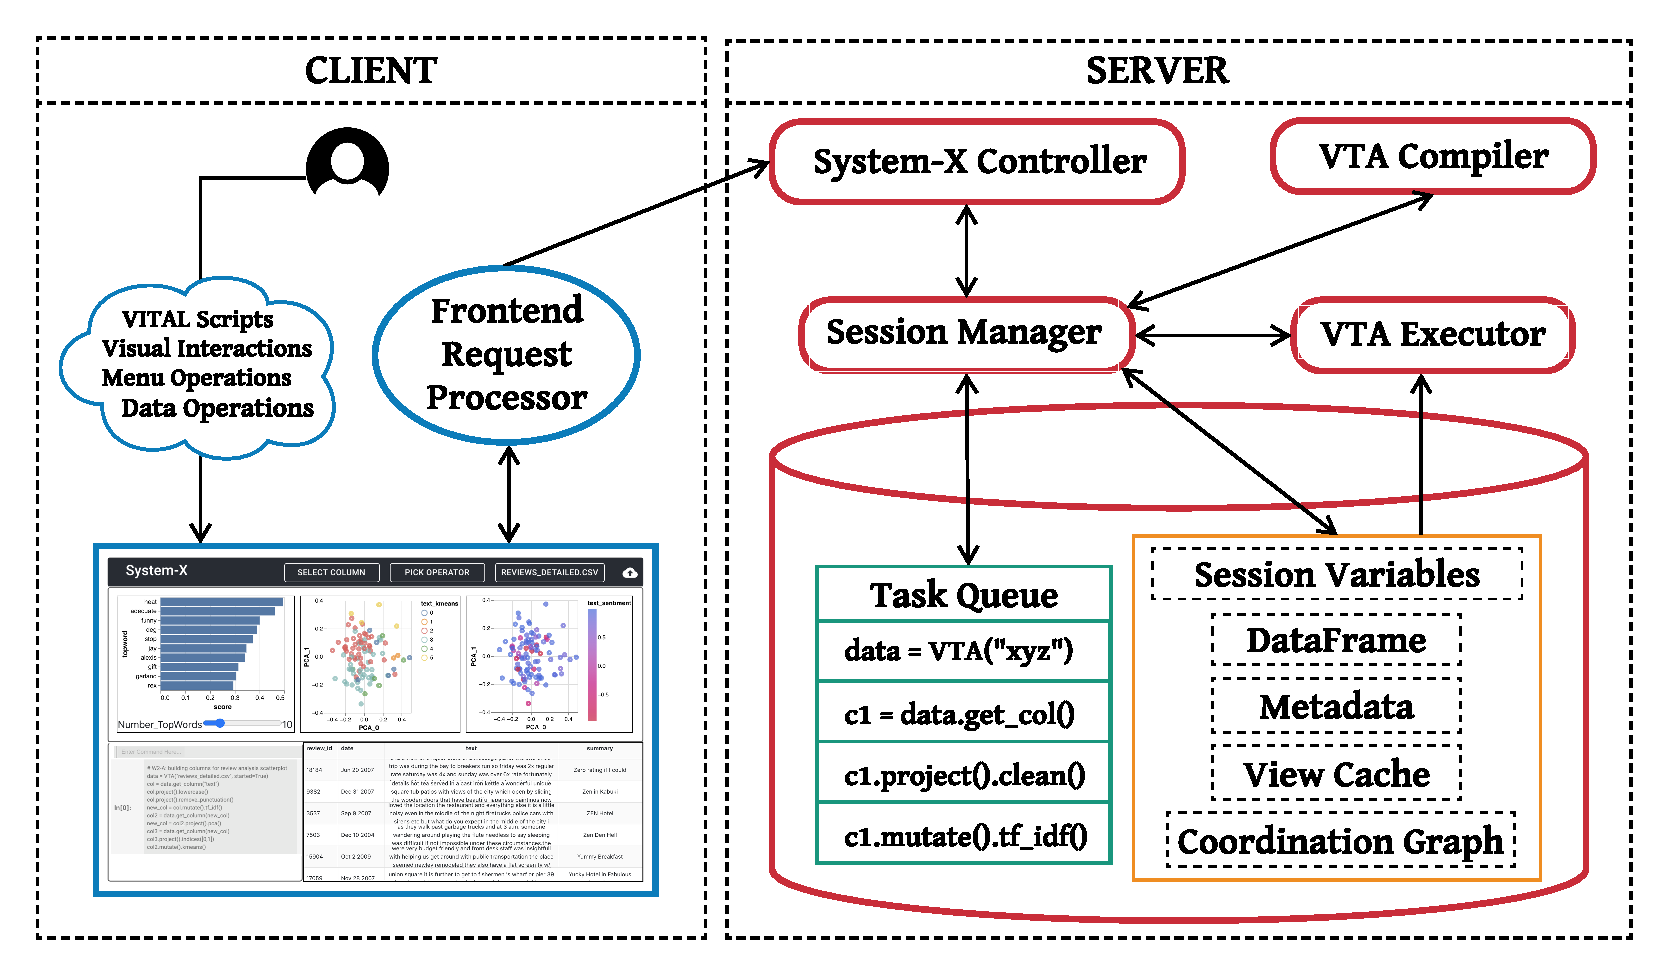
\includegraphics[width=\linewidth]{figures/leam_arch.pdf}
  \caption{\small \system architecture.\todo{Repeat the most important architectural design goals.} \label{fig:arch}} 
  %\vspace{-20pt}
\end{figure}


We depict the architecture
diagram in Figure~\ref{fig:arch}.
On the client or front end side,
the \system client is responsible
for capturing user input 
on various interface components,
and for rendering the views
based on results returned by the
back-end. Examples of user interactions include
\vital commands in Code Editor, 
operator selection in Operations Menu operator,
interaction with Data View and charts in Chart View.
Given any user interaction
on the front end,
the \system Request Processor
issues a request to the backend \system Controller.
This controller manages the uploaded data and sessions
while propagating user interactions to the {\em session
manager}. 

The session manager interprets the user 
interaction---any interactions on the Operations Menu
is sent to a lightweight \vta Compiler~\cite{rahman2020leam}
while the \vital commands on the Code Editor are pushed in a task queue.
The \vta compiler translates the user-selected operator to a \vital
command which is then executed by the \vta Executor. 
Since users can either write single- or multi-line \vital commands,
\system backend employs a Task Queue to keep track of the sequence of
tasks. Whenever the \vta executor completes the execution of a \vital command, the session 
manager fetches an unprocessed command from the task queue and sends that to the
executor. The \vta executor leverages the python runtime to access any global or local variables in the session and executes the command on the desired data.

\system backend utilizes a customized dataframe called \vitaframe for enabling text data analysis~\cite{rahman2020leam} operations. \vitaframe columns are complex objects that not only contains the raw data, but also the schema of the column, associated metadata and the metadata schema type. For example,
in Figure~\ref{fig:workflow}a, in the third cell of the Code Editor, the user computes the \code{tf\_idf} feature vector of the review column, and adds the vector as a new column. As a byproduct of this operation, a dictionary of unique words called ``feature\_label'' is created which is a metadata of the newly created column. The dictionary metadat is later utilized to create a bar chart of top ranked words (Figure~\ref{fig:workflow}a fourth cell).
Such a column specification with schema is necessary to validate a \vta operation. \system session manger also employs a View Cache to track states of the front end components and always remains in sync with the front end. If the states of a component is updated after a \vital command execution, the changes are propagated to the front end. Also, \system employs a Coordination Graph to manage coordination among linked views. For each view in the front end, \system maintains an adjacency list---for any interaction on a view, all the views in its adjacency list are updated. For example, selecting a bar in the barchart in Figure~\ref{fig:chartview_coordinate_multi} updates the scatterplot and Data View in its adjacency list.

